\documentclass[12pt,a4paper,bibliography=totocnumbered]{scrartcl}
\usepackage[ngerman]{babel}

\usepackage{graphicx}
\usepackage{geometry}
%\usepackage{titlesec}
\usepackage{fancyhdr}
\usepackage[pdfpagelabels=true]{hyperref}
\usepackage{xcolor}
\usepackage{listings}
\usepackage[T1]{fontenc}

\definecolor{mGreen}{rgb}{0,0.6,0}
\definecolor{mGray}{rgb}{0.5,0.5,0.5}
\definecolor{airforceblue}{rgb}{0.36, 0.54, 0.66}
\definecolor{amber}{rgb}{1.0, 0.49, 0.0}
\definecolor{coolgrey}{rgb}{0.55, 0.57, 0.67}
\definecolor{davy}{rgb}{0.33, 0.33, 0.33}
\definecolor{backgroundColour}{rgb}{0.95,0.95,0.95}

\lstdefinestyle{CStyle}{
    backgroundcolor=\color{backgroundColour},   
    commentstyle=\color{davy},
    keywordstyle=\color{amber},
    numberstyle=\tiny\color{mGray},
    stringstyle=\color{airforceblue},
    basicstyle=\footnotesize,
    breakatwhitespace=false,         
    breaklines=true,                 
    captionpos=b,                    
    keepspaces=true,                 
    numbers=left,                    
    numbersep=5pt,                  
    showspaces=false,                
    showstringspaces=false,
    showtabs=false,                  
    tabsize=2,
    language=C
}

\geometry{a4paper, top=27mm, left=25mm, right=25mm, bottom=35mm, headsep=10mm, footskip=12mm}

\makeatletter
\renewcommand\@biblabel[1]{}
\makeatother
%__________________________________________________________________

\begin{document}

%\titlespacing{\section}{0pt}{12pt plus 4pt minus 2pt}{-6pt plus 2pt minus 2pt}

% Kopf- und Fusszeile
\pagestyle{fancy}
\renewcommand{\sectionmark}[1]{\markright{\arabic{section}.\ #1}}
\renewcommand{\leftmark}{}
\fancyhf{}
\lhead{}
\chead{}
\rhead{\thesection\space\contentsname}
\lfoot{Abgabe 4}
\cfoot{}
\rfoot{\ \linebreak  \thepage}
\renewcommand{\headrulewidth}{0.4pt}
\renewcommand{\footrulewidth}{0.4pt}

%______________________________________________________________________


%______________________________________________________________________

\clearpage

% Arabische Seitenzahlen
\pagenumbering{arabic}
\setcounter{page}{1}

% Geändertes Format für Seitenränder, arabische Seitenzahlen
\fancyhead[LE,RO]{\rightmark}
%\fancyhead[LO,RE]{\leftmark}
\fancyfoot[LE,RO]{\thepage}

%______________________________________________________________________

\section*{Abgabe 4}

Das main-Programm startet zwei Threads.
Thread 1 wird alle 4ms aktiv und arbeitet dann für 2ms. Alle drei Takte setzt Thread 1 nach seiner Verarbeitungszeit dann eine Semaphore, auf die Thread 2 wartet.
Thread 2 wartet auf eine Semaphore. Sobald diese frei ist, arbeitet er für 3ms.

\begin{lstlisting}[style=CStyle]
#include <stdlib.h>
#include <stdio.h>
#include <pthread.h>
#include <semaphore.h>
#include <unistd.h>
#include <string.h>
#include <errno.h>

#define BILLION  1000000000L

sem_t semaphore;

void oneSecMethod() {
	volatile int zero = 0, one = 1, sum;
	int i;
	for (i = 0; i < 50000; i++) {
		sum = zero + one;
	}
	for (i = 0; i < 50000; i++) {
		sum = zero + one;
	}
}

void waste_msecs(unsigned int msecs) {
	int i;
	for (i = 0; i < msecs; i++) {
		oneSecMethod();
	}
}
void do_nothing() {
	;
}

/**
* Zaehlt Zeit um 4ms nach oben.
* Rechnet 2ms.
* Schlaeft bis die anfaenglichen 4ms vorbei sind.
* Alle 3 Durchlaeufe wird eine Semaphore freigegeben.
*/
void* function_thread1(void* arg) {
	struct timespec time;
	int i, err;

	if (clock_gettime(CLOCK_REALTIME, &time) == -1) {
		perror("clock gettime");
		return (void *) EXIT_FAILURE;
	}

	while (1) {

		time.tv_nsec += 4 * 1000 * 1000;

		if (time.tv_nsec >= BILLION) {
			time.tv_nsec = time.tv_nsec % BILLION;
			time.tv_sec += 1;
		}

		waste_msecs(2);

		err = clock_nanosleep(CLOCK_REALTIME, TIMER_ABSTIME, &time, NULL);
		if (err != 0) {
			printf("clock nanosleep: %s \n", strerror(err));
		}
		if (i == 3) {
			sem_post(&semaphore);
			i = 0;
		}
		++i;
	}

	return NULL;
}

/**
* Wartet auf Freigabe einer Semaphore.
* Arbeitet dann 3ms.
*/
void* function_thread2(void* arg) {
	while (1) {
		while (sem_wait(&semaphore) && (errno == EINTR))
			;
		waste_msecs(3);
	}
	return NULL;
}

int main(int argc, char *argv[]) {
	pthread_t thread_one;
	pthread_t thread_two;
	pthread_attr_t attr;
	pthread_attr_t attr2;
	int err;

	struct sched_param param;

	param.sched_priority += 12;

	pthread_attr_init(&attr);
	pthread_attr_init(&attr2);

	pthread_attr_setschedparam(&attr, &param);
	pthread_attr_setdetachstate(&attr, PTHREAD_CREATE_JOINABLE);
	pthread_attr_setdetachstate(&attr2, PTHREAD_CREATE_JOINABLE);

	err = pthread_attr_setinheritsched(&attr, PTHREAD_EXPLICIT_SCHED);

	if (err != 0) {
		printf("pthread_attr_setinheritsched: %s ", strerror(err));
	}

	sem_init(&semaphore, 0, 1);

	err = pthread_create(&thread_one, &attr, &function_thread1, NULL);

	if (err != 0) {
		printf("pthread_create: %s ", strerror(err));
	}

	err = pthread_create(&thread_two, &attr2, &function_thread2, NULL);

	if (err != 0) {
		printf("pthread_create: %s ", strerror(err));
	}

	err = pthread_join(thread_one, NULL);

	if (err != 0) {
		printf("pthread_create: %s ", strerror(err));
	}

	err = pthread_join(thread_two, NULL);

	if (err != 0) {
		printf("pthread_create: %s ", strerror(err));
	}

	return EXIT_SUCCESS;
}
\end{lstlisting}

\begin{figure}[h]
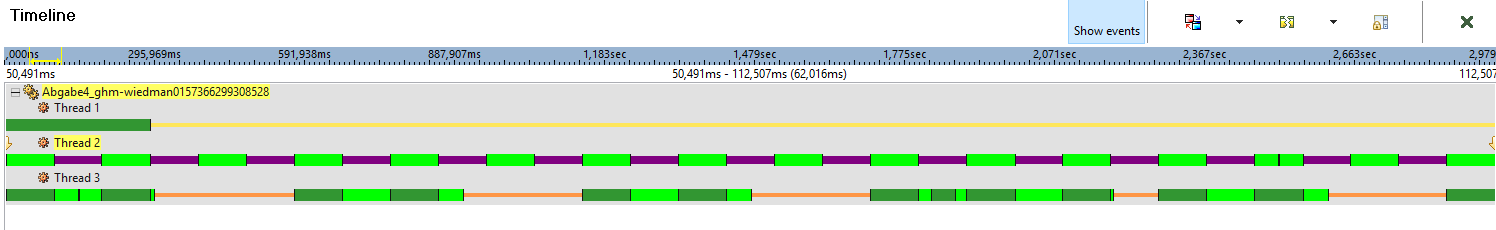
\includegraphics[width=\textwidth]{bilder/QNX_A4}
\centering
\end{figure}
Thread 1(im Bild Thread2) hat eine höhere Priorität als Thread 2(im Bild Thread3), da sonst Thread 1 seinen 4ms Rhythmus nicht einhalten kann. Thread 1 verdrängt Thread 2 und hält somit seinen Rhythmus ein.

\begin{figure}[h]
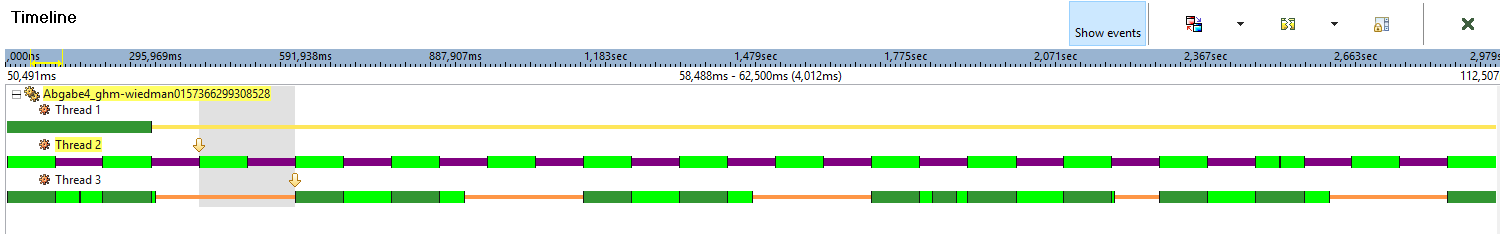
\includegraphics[width=\textwidth]{bilder/QNX_A4_1}
\centering
\end{figure}
%______________________________________________________________________

\end{document}












